\chapter{Implementation}\label{chap:implementation}

\section{Work plan: work packages, deliverables}

\subsection*{Overall structure of the work plan}

Our work plan is divided into seven scientific work packages.  The
first group of work packages is dedicated to the networking activities
that are needed to gather the proofs today located in different
libraries.  The second to making these proofs accessible, beyond
trans-national and virtual access.  The third to joint research
activities that prepare the future of Logipedia.

Together with these seven scientific work packages, two more work
packages are dedicated to dissemination, communication and
exploitation and to management.

\begin{longtable}{|p{0.05\textwidth}|p{0.15\textwidth}|p{0.17\textwidth}|p{0.55\textwidth}|}
\hline
\rowcolor{color2}\multicolumn{4}{|l|}{\bf Networking activities:}\\
\hline
WP1
&
Integration &
Jesper Cockx

(Delft)
&
Instrument the systems for which we already know how to encode the
proofs in Dedukti, and make these proofs available in Logipedia.
\\
\hline
WP2
&
Automatic theorem proving
&
Chantal Keller

(Saclay)
& 
Develop automatic theorem provers to populate,
help, and benefit from Logipedia.
\\
\hline
WP3
&
Large libraries
&
Tobias Nipkow

(M\"unchen)
&
Export large dedicated libraries in curated form 
to Logipedia for end-user applications.
\\
\hline
\end{longtable}

\begin{longtable}{|p{0.05\textwidth}|p{0.15\textwidth}|p{0.17\textwidth}|p{0.55\textwidth}|}
\hline
\rowcolor{color2}\multicolumn{4}{|l|}{\bf Trans-national and virtual access:}\\
\hline
WP4
&
Access
&
Frédéric Blanqui

(Inria)
&
Define and build the Logipedia hardware and software infrastructure in
which the proofs will be integrated.
\\
\hline
WP5
&
Structure of the encyclopedia
&
Florian Rabe

(Erlangen)
&
Provide infrastructure for the structured ontological representation
of libraries and use it to enrich the information about formal
libraries in Logipedia.
\\
\hline
\end{longtable}


\begin{longtable}{|p{0.05\textwidth}|p{0.15\textwidth}|p{0.17\textwidth}|p{0.55\textwidth}|}
\hline
\rowcolor{color2}\multicolumn{4}{|l|}{\bf Joint research activities:}\\
\hline
WP6
&
Theories
&
Cezary Kaliszyk

(Inssbruck)
&
Bringing proof systems implementing a theory 
that has not yet been expressed in Dedukti to LIL 2 or better.
\\
\hline
WP7
&
Proof engineering
&
Filip Marić

(Belgrade)
&
Investigate methods for detecting concept alignments and apply
them to build a library of alignments present across the Logipedia database.
\\
\hline
\end{longtable}

\begin{longtable}{|p{0.05\textwidth}|p{0.15\textwidth}|p{0.17\textwidth}|p{0.55\textwidth}|}
\hline
\rowcolor{color2}\multicolumn{4}{|l|}{\bf Dissemination, communication, exploitation, and management:}\\
\hline
WP8
&
Dissemination, communication, and exploitation
&
Pascal Fontaine

(Liège)
&
Expand the use of Logipedia in research, industry, education, and publishing.
\\
\hline
WP9
&
Management
&
Gilles Dowek

(Inria)
&
Coordinate this large community, in a benevolent atmosphere, for optimal
efficiency.
\\
\hline
\end{longtable}

These work packages are diverse in the number of tasks and
partners. Some of them are large, while others are smaller. This
reflects the diversity of their natures and goals. The work package
``access'' for instance has a very definite and critical goal, it must
have a small number of partners and be focused on its goal. In
contrast, the work package ``theories'' requires experts in many
different systems.  It therefore has a larger number of partners.

{\color{red} Read objectives of WP: they must be objectives}



\subsection*{Detailed work description}

\begin{workplan}

% the template says: "indicate in the work package title the type of activity"

  \newcommand\na{(Networking activity)}
  \newcommand\tnva{(Trans-national and virtual access)}
  \newcommand\jra{(Joint research activity)}
  \newcommand\titlewp[3]{\bigskip\noindent\colorbox{color3}{\begin{minipage}\textwidth\bf Work Package #1: #2\end{minipage}}\input{workpackages/#3}}

\titlewp{1}{Integration \na}{instrumentation}

\titlewp{2}{Automatic theorem provers \na}{atpetc}

\titlewp{3}{Large libraries \na}{libraries}

\titlewp{4}{Accesses to the encyclopedia \tnva}{access}

\titlewp{5}{Structure of the encyclopedia \tnva}{structuring}

\titlewp{6}{Theories \jra}{theories}

\titlewp{7}{Proof engineering \jra}{alignment}

\titlewp{8}{Dissemination, communication and exploitation}{dissemination}

\titlewp{9}{Management}{management}

\end{workplan}

\subsubsection*{List of all deliverables}\label{sec:deliverables}

Here is an overview of the deliverables 
of the work packages. 

%In the table below, \emph{integrating work deliverables} (see top of
%section~\ref{sec:wplist}) are printed in boldface to mark them. They integrate
%contributions from multiple work packages.

{\footnotesize\inputdelivs{8cm}}

%%% Local Variables: 
%%% mode: latex
%%% TeX-master: "propB"
%%% End: 


\subsection*{Timing of the different work packages and their components}

\makeatletter
\newcounter{month}
\setcounter{month}{0}\@whilenum\value{month}<\numexpr\pdataref@aux{prop}{gen}{months}+1\do{\expandafter\newlength\csname offset\the\value{month}\endcsname\stepcounter{month}}
\def\offset@reset#1{\setcounter{month}{0}\@whilenum\value{month}<\numexpr\pdataref@aux{prop}{gen}{months}+1\do{\expandafter\setlength\csname offset\the\value{month}\endcsname{#1}\stepcounter{month}}}
\def\offset@incr#1#2{\expandafter\addtolength\csname offset#1\endcsname{#2}}
\def\offset@get#1{\expandafter\the\csname offset#1\endcsname}

\begin{ganttchart}
[
vgrid=true,
hgrid=true,
title height=1,
y unit title=\baselineskip,
y unit chart=.6\baselineskip,
x unit=10pt,
group peaks width=0,
group peaks height=0,
group left shift=0,
group right shift=0,
group top shift=.25,
group height=.5,
group/.append style={fill=blue},
group label node/.append style={font=\bf},
bar top shift=.25,
bar height=.5,
bar/.append style={fill=green,rounded corners=3pt,draw opacity=0},
bar label node/.append style={font=\footnotesize},
milestone left shift=.5,
milestone right shift=.5,
milestone top shift=0,
milestone height=1,
milestone/.append style={fill=yellow},
milestone inline label node/.append style={font=\scriptsize},
vrule/.style={very thick,red},
]
{1}{\pdataref@aux{prop}{gen}{months}}
\pgfdeclarelayer{delivs}
\pgfdeclarelayer{miles}
\pgfsetlayers{background,main,miles,delivs}
\gantttitle{\makebox[0pt][r]{\textbf{\textit{Month\ }}}}{0}
\gantttitlelist[title label node/.append style={font=\scriptsize}]{1,...,\pdataref@aux{prop}{gen}{months}}{1}
\edef\@wps{\pdataref@aux{all}{wp}{ids}}
\@for\@wp:=\@wps\do{
\\\\
\ganttgroup{\pdataRef{wp}{\@wp}{label}}{\pdataref@num{wp}{\@wp}{start}}{\pdataref@num{wp}{\@wp}{end}}
\begin{pgfonlayer}{delivs}
\offset@reset{.5pt}
\edef\@delivs{\pdataref@aux{\@wp}{delivs}{ids}}
\@for\@deliv:=\@delivs\do{
\ifodd\pdataref@num{deliv}{\@deliv}{due}
\ganttmilestone[inline,milestone inline label node/.append style={above right=0pt and -15pt}]{\pdataRef{deliv}{\@deliv}{label}}{\pdataref@num{deliv}{\@deliv}{due}}
\else
\ganttmilestone[inline,milestone inline label node/.append style={below right=\offset@get{\pdataref@num{deliv}{\@deliv}{due}} and -15pt}]{\pdataRef{deliv}{\@deliv}{label}}{\pdataref@num{deliv}{\@deliv}{due}}
\offset@incr{\pdataref@num{deliv}{\@deliv}{due}}{.6\baselineskip}
\fi
}
\end{pgfonlayer}
\\
\edef\@tasks{\pdataref@aux{\@wp}{task}{ids}}
\@for\@task:=\@tasks\do{
\\
\edef\@wphases{\pdataref@safe{task}{\@task}{wphases}}
\@for\@wphase:=\@wphases\do{
\decode@wphase\@wphase
\ganttbar{\pdataRef{task}{\@task}{shorttitle}}{\wphase@start}{\wphase@end}
}
}
}
\begin{pgfonlayer}{miles}
\offset@reset{0pt}
\edef\@miles{\pdataref@aux{all}{mile}{ids}}
\@for\@mile:=\@miles\do{
\ganttvrule[vrule label node/.append style={below=\offset@get{\pdataref@num{mile}{\@mile}{month}}}]{\pdataRef{mile}{\@mile}{label}}{\pdataref@num{mile}{\@mile}{month}}
\offset@incr{\pdataref@num{mile}{\@mile}{month}}{\baselineskip}
}
\edef\@meetings{1,16,32,48}
\@for\@meeting:=\@meetings\do{
\ganttvrule[vrule/.append style={orange}]{general meeting}{\@meeting}
}
\end{pgfonlayer}
\end{ganttchart}
\makeatother

\subsection*{Relation between the components}

Two work packages are critical for the success of the project, the
work package 4, that aims at building the software infrastructure of
Logipedia and the work package 1 that aims at populating it with proofs.
All the other work packages depend of these two.

Finally all the workpackages contribute to just one goal: interoperability,
sustainability, and cross-verification of formal proofs.

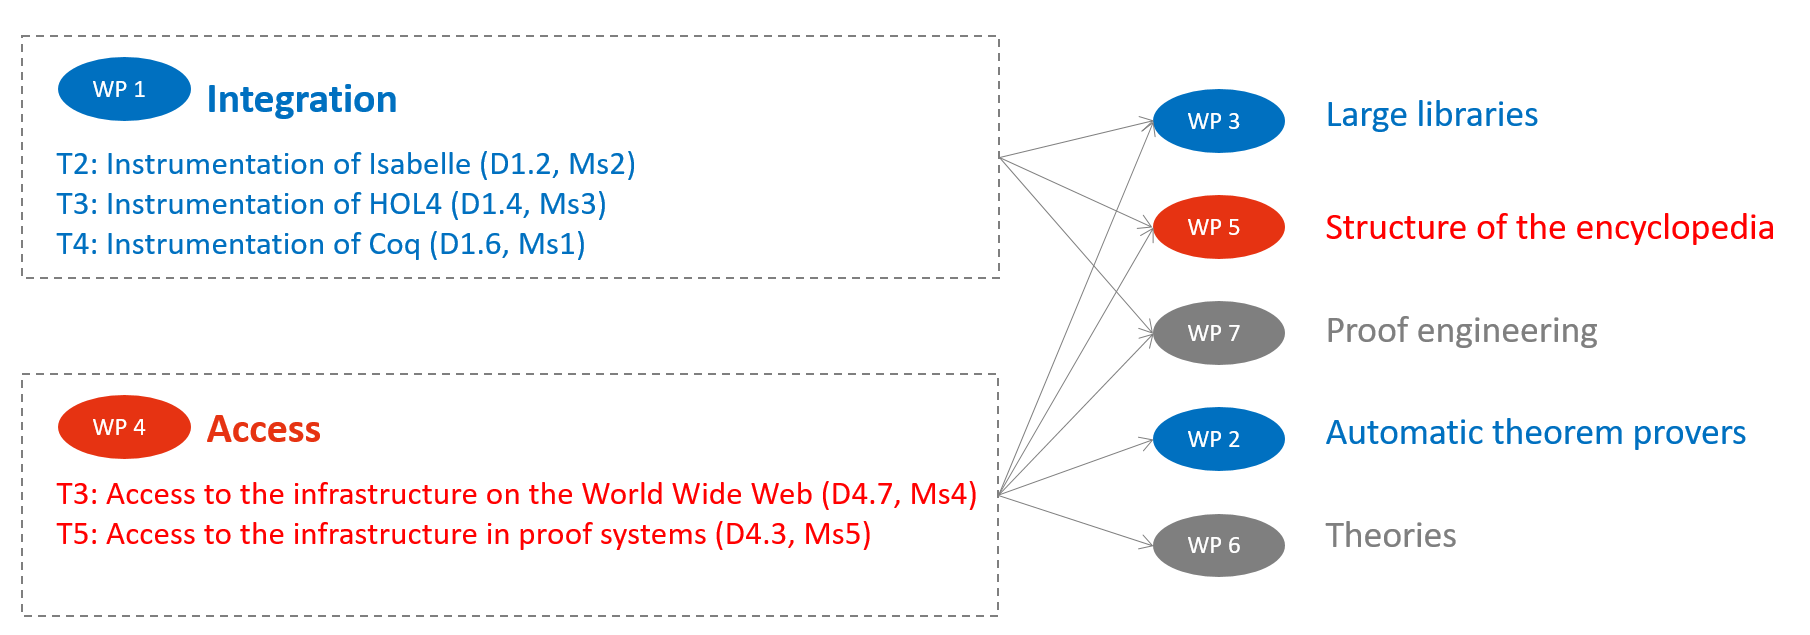
\includegraphics[width=\textwidth]{img/PERT}


%%% Local Variables:
%%%   mode: latex
%%%   mode: flyspell
%%%   ispell-local-dictionary: "english"
%%% End:


%%%%%%%%%%%%%%%%%%%%%%%%%%%%%%%%%%%%%%%%%%%%%%%%%%%%%%%%%%%%%%%%%%%%%%%%%%%%%%
\section{Management structure, milestones and procedures}

The Logipedia consortium will gather twenty-eight beneficiaries and partners
from eleven European countries during four years. The project management
structure will be tailored to the specificities and needs of this
large consortium and its ongoing network development.

%%%%%%%%%%%%%%%%%%%%%%%%%%%%%%%%%%%%%%%%%%%%%%%%%%%%%%%%%%%%%%%%%%%%%%%%%%%%%%
\subsection{Organisational structure}

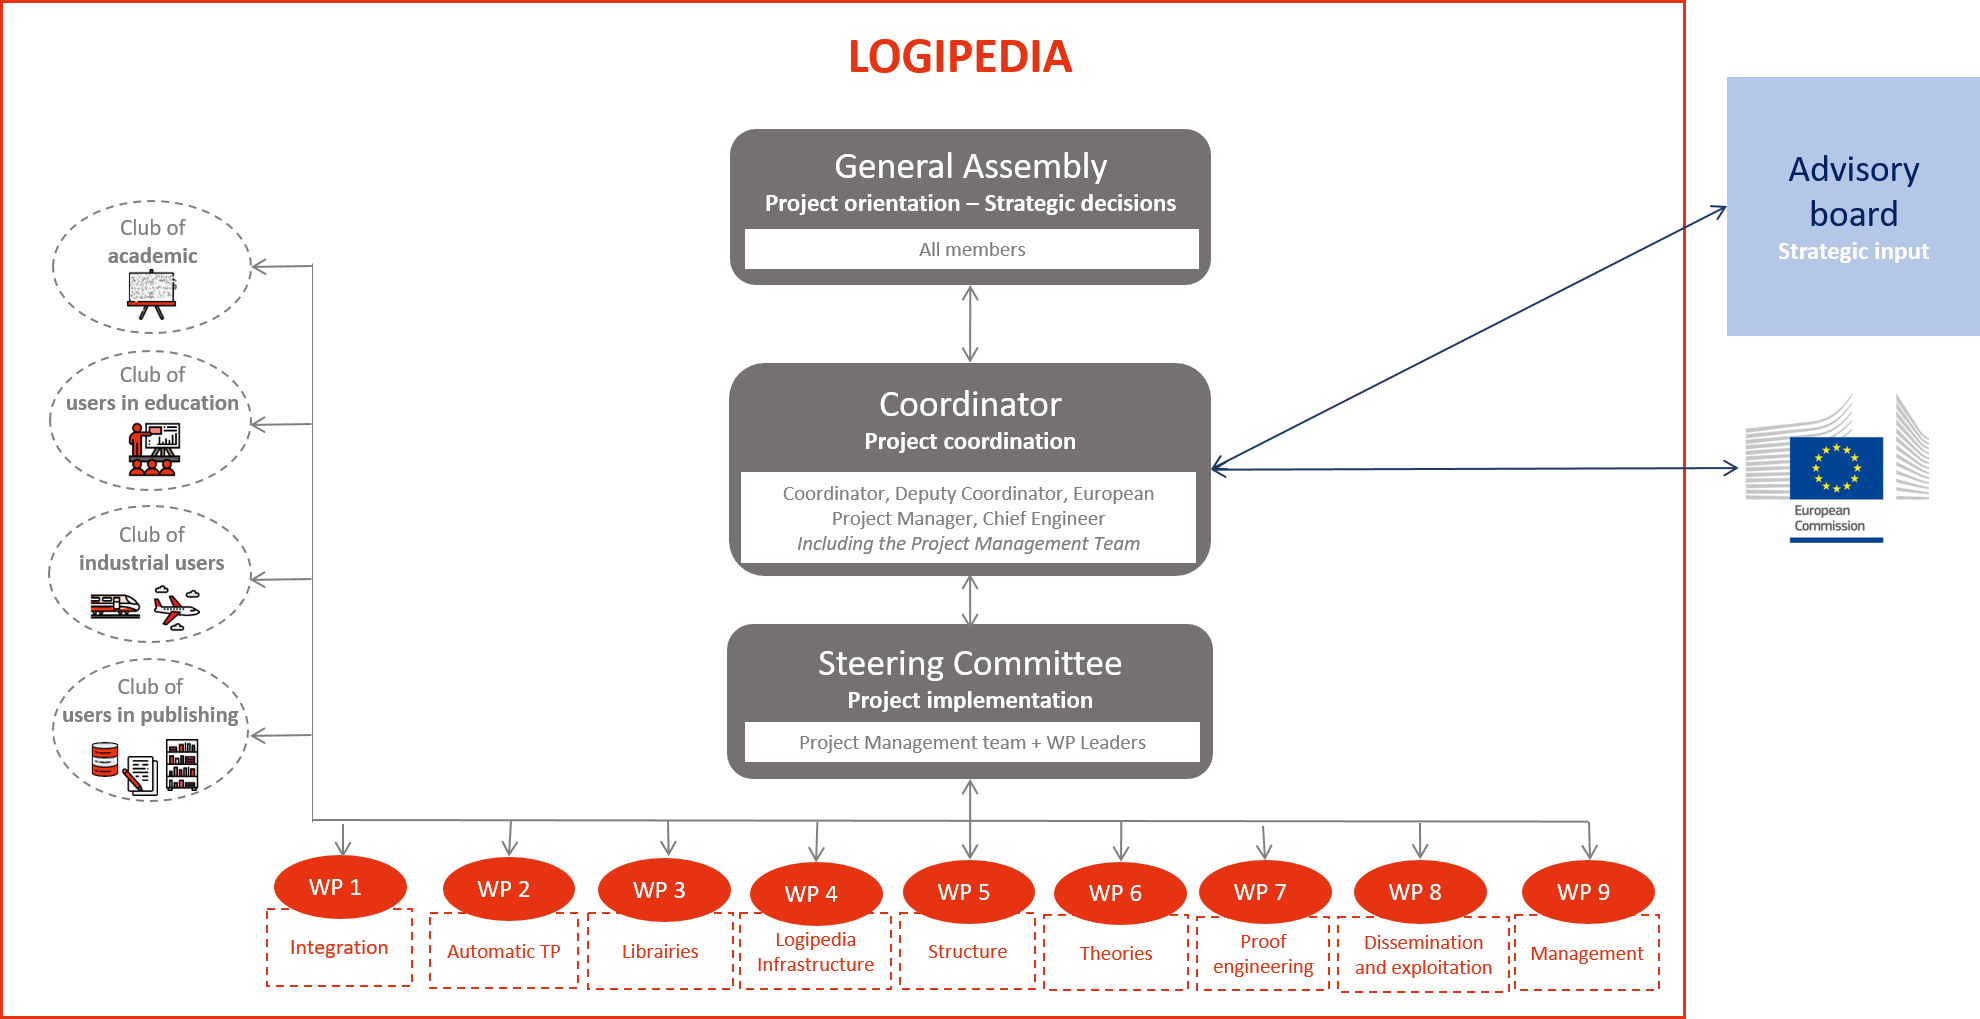
\includegraphics[width=\textwidth]{img/Gouvernance}

In this picture add the EC (talks to Coordinator only)

vice coordinator -> Deputy coordinator

Names of WP

Place of the cooddinator : outside of the bulbe talks to the SN

General assembly talks to SC (and not the SC is part of it)


\subsubsection*{The project management team}

\begin{compactitem}
\item{\bf The Coordinator}: the 
coordinator is responsible for the coordination of
scientific and technical activities in order to meet the objectives
set by the European Commission in the Grant Agreement. The 
coordinator works closely with the work package leaders
within the steering committee, in order to monitor the progress of the
scientific and technical work and identify potential risks within each
work package. The coordinator will daily
collaborate with the European project manager in charge of the
day-to-day management of Logipedia. The project will be managed by Pr
Gilles Dowek, permanent senior researcher at Inria Saclay. He will
also chair the meetings of both the general assembly and steering
committee.

\item{\bf The Deputy Coordinator}: The Deputy coordinator, Frédéric
Blanqui, seconds and replaces the coordinator if needed.

\item{\bf The European Project Manager}: The European project manager
  is a team member of the Technology Transfer and Partnership Office
  of Inria Saclay. He or she is in charge of all administrative,
  financial and legal management tasks as listed in
  \WPref{management}. The European project manager is the interface
  between the project and the European Commission as it represents the
  point of contact for the European Commission. The European project
  manager has the overall administrative and financial responsibility
  for the organisation and administrative and financial monitoring of
  the project.

\item{\bf The Chief Engineer}: The chief engineer is an experienced
research engineer from Inria Saclay and is responsible for ensuring
the development and maintenance of tools at Inria Saclay and
supervising the development tasks achieved at the other
beneficiaries. The chief engineer will ensure the coherence of the
Logipedia tools development, according to the defined schedule in the
Grant Agreement.
\end{compactitem}

Innovation management and intellectual property rights issues will be
handled by the European project manager, supported by the experienced
Technology Transfer and Partnerships Office of Inria Saclay. The
project management team will establish appropriate policies and rules
for the management of intellectual property rights for the knowledge
developed within the project, as well as the identification of the
opportunities for the exploitation of the project results in
innovation activities. Issues related to innovation and/or
intellectual property rights management will be tackled at every
steering committee meeting.

\subsubsection*{The operational level}

\begin{compactitem}
\item{\bf The Steering Committee}: The steering committee is composed
  of the Coordinator, the Deputy coordinator, the chief engineer, the
  European project manager and the work package leaders. The steering
  committee is the supervisory body for the implementation of the
  project. The steering committee is responsible innovation,
  intellectual property, and for monitoring the activities of the
  project and the implementation of decisions taken by the general
  assembly. It can formulate proposal for changes in the description
  of action and the related consortium budget. Those changes will have
  to be agreed by the general assembly first and then the European
  commission. The steering committee is chaired by the coordinator.

\item{\bf The Work Package Leaders}: The work package leaders are
responsible for the monitoring and management of the activities and
results within their work packages. In particular, work package
leaders i) identify deviations from the project plan and report them
to the steering committee, ii) manage and supervise the preparation of
reports and their timely delivery, iii) control and monitor activities
of tasks and regularly meet once per month with task leaders, iv)
manage the information flow with other work packages via the steering
committee.

\item{\bf The Task Leaders}: The task leaders are responsible for
coordinating the scientific and technical work in their task and
making the day to day technical decisions that solely affect their
task. Inter-task decisions are coordinated with the work package
leaders.

\item{\bf The Club Leaders}: The club leaders are in charge of
disseminating of the tools developed by the Logipedia consortium in
various communities. They organize the activity of the club. They give
ongoing feedback to the consortium during the course of the project.
\end{compactitem}

\subsubsection*{The strategic level}

\begin{compactitem}
\item{\bf The General Assembly}: The general assembly is composed by all
the members of the consortium, with each representative having one
vote. Every new partner will have a voting right. The general assembly
will gather at least once a year, and as many virtual meetings as
needed. The general assembly is the main governance and ultimate
decision-making body of the consortium. The general assembly must
review the project progress, decide on contingency actions in case of
deviations from the plan and take final decisions on policy and
contractual issues and conflicts as requested by the steering
committee.

\item{\bf The Advisory Board}: The advisory board is a consultation body to
the steering committee and general assembly. It will bring external
and non-legally binding perspective on the scientific and technical
development of the project, ecosystem building and the future of the
encyclopedia. The advisors of this board will attend the yearly
general assembly plenary meeting and will be consulted on the strategy
of the project. The advisory board should aim at representing the
stakeholders of the Logipedia ecosystem without including any
beneficiary or associate partner’s employees. It will be composed of,
among others, industrial and international academic partners
(including non-European ones) apointed by the coordinator after
consulting the steering committee. To start with, we suggest to
include: June Andronick (Data61, Kensington NSW, AU), Denis Cousineau
(Mitsubishi Electric R\&D Centre Europe, FR), Thomas Letan (ANSSI, FR),
Jacques Fleuriot (University of Edinburgh, UK), Natarajan Shankar
(SRI, US), Aaron Stump (Iowa University, US), Laurent Voisin
(Systerel, FR).
\end{compactitem}

\subsubsection*{Internal communication and collaborative ecosystem}

The communication of the consortium including their internal tools is
managed in task 10.2.  The consortium will make use of a number of
project management tools, such as a visio conferencing tool, a project
repository to have an updated account of the project’s important
documents, the progress of the work packages work and deliverables,
all the advances in the project and all the meetings minutes, mailing
lists, etc. that facilitate the smooth execution of the project. This
collaboration environment will be provided by the coordinator of the
project.

Work packages, chaired by work package leaders, will have monthly
planned visio conferences and meetings as need by the work plan;
additional technical meetings may be set up by task leaders or
individual partners. The steering committee will have monthly visio
conferences and will meet twice a year. Dedicated working groups will
be planned as needed according to the work plan.  All meetings will be
documented by minutes listing major decisions and action items.

The project management team will be in charge of all organisational
issues in the general assembly meetings, supported by the local
partner. The project will organise meetings of the general assembly at
least once a year. To equally share travel costs among partners,
physical meetings will be located by rotation at partners’
locations. Project review meetings will be done on a regular basis
according the Grant Agreement provisions.

%%%%%%%%%%%%%%%%%%%%%%%%%%%%%%%%%%%%%%%%%%%%%%%%%%%%%%%%%%%%%%%%%%%%%%%%%%%%%%
\subsection{Decision-making Process}

Our approach for the decision-making process is to locate the decision
as close as possible to the level responsible for the execution (from
task to general assembly level). Decisions are managed within
frequent project meetings, either on-site or via
teleconference. Decisions can be also managed by consultation. If
voting is needed, the agenda should clearly indicate this fact. Quorum
and voting rules will be defined in the Consortium
Agreement. Decisions are binding once the relevant part of the meeting
minutes has been accepted. Any changes to the project plan and scope
must be reviewed and approved by all levels of project management,
before proposing these changes to the steering committee and any
modifications will be considered rejected, after rejection on any of
these involved levels.

Another guiding principle is to avoid conflicts. Nevertheless, should
one arise, a conflict resolution will be ready to be put in place to
deal with it accordingly. The conflict resolution foresees that each
conflict will be mediated, solved or decided at the lowest level
possible. Attempts to solve issues within the consortium will be
carried out in increasing order of authority first at task level
(management of task leader), work package level (management of work
package leaders), and then following the management bodies till the
general assembly. Further rules related to conflict resolutions will
be laid out in the Consortium Agreement.

%%%%%%%%%%%%%%%%%%%%%%%%%%%%%%%%%%%%%%%%%%%%%%%%%%%%%%%%%%%%%%%%%%%%%%%%%%%%%%
\subsection{Monitoring and reporting}

\subsubsection*{Internal reporting}

The project management team continuously monitors the project plan
with its milestones. Each work package leader will be
responsible for the correct execution of the implementation plan for
the corresponding work package. In terms of reporting, this means the work package leaders
will be in charge of gathering the information related to their own
work packages.

Regular audio-conferences of the Steering Committee are foreseen,
which allows work package leaders to identify risks and
discuss them together. This ensures that management (coordination,
European project manager) is aware of potential problems and
deviations and can initiate countermeasures long before a situation
becomes critical. This ensure to spot the blocking points and implements
the solution at the right time.


In case there is a deviation from the work plan, the 
coordinator will initiate corrective actions through the
task leader and the work package leader. The work package leader will
be responsible to implement these actions in dialogue with the
different partners involved in their work packages.

\subsubsection*{Reporting to the European Commission}

The Logipedia consortium will follow the mandatory reporting period
required by the European Commission. 

The project management team will provide the necessary templates in
order to achieve the reporting in due time. Work package leaders will
be asked to gather the relevant information provided by the task
leader regarding their work package and to summarise in order to be
reviewed by the steering committee. It will then be treated by the
coordinator and European project manager and sent to the
European Commission.

%%%%%%%%%%%%%%%%%%%%%%%%%%%%%%%%%%%%%%%%%%%%%%%%%%%%%%%%%%%%%%%%%%%%%%%%%%%%%%
\subsection{Significant risks and associated contingency plans}
\label{sec:risks}

\subsubsection*{Scientific risks}

\begin{longtable}{|p{0.30\textwidth}|p{0.10\textwidth}|p{0.50\textwidth}|}
\hline
{\bf Description of the risk}
&
{\bf Work packages involved}
&
{\bf Proposed measure of mitigation}
\\
\hline
Some theories are difficult to express in Dedukti.
(Probability: medium. Severity: low.)

{\color{red} It is not that it is difficult that is a risk, it is
that we fail to do it}
&
WP6
&
We have carefully divided the systems into two groups: those that do not
present risks (WP1) and those that do (WP6). The success we got with the
theories implemented in systems of the first group gives us confidence
that the theories implemented in those of the second can also be
expressed in Dedukti.  If one of them happens to be more difficult, we
can still build a large encyclopedia with the systems of the first
group. We can also extend Dedukti so that it can express more theories,
as we have already done in the past.
\\
\hline
Some libraries require too much time and memory
to be expressed in Dedukti (Probability: medium. Severity: low.)
&
WP3
&
There are several ways to mitigate this risk: optimize the
representation of data (sharing, elimination of redundancies, etc.), 
use faster and larger computers. This may also mean that some tasks
of this work package are premature and that we have to wait for
faster computers, that Moore's law will provide.
\\
\hline
No adoption from the community. (Probability: low. Severity: high.)
&
All 
&
The community may fail to adopt Logipedia for several reasons. Because
of a problem of design of Logipedia, in which case we will have to
understand what needs to be changed in a second version.  It may be
because the Logipedia community is too small.  This explains that we
have decided to include twenty-eight partners in the project.  It may
also be because of an insufficient dissemination activity.  This is
why we propose to create the four clubs of users and we will devote
time and energy to the animation of these clubs, together with other
dissemination activities, such as summer schools and conferences.
\\
\hline
\end{longtable}

\subsubsection*{Management risks}

\begin{longtable}{|p{0.30\textwidth}|p{0.10\textwidth}|p{0.50\textwidth}|}
\hline
Brexit disrupts the project (Probability: low. Severity: medium.)
&
All (specially WP6, WP7)
&
As we have two partners from the United Kingdom, Brexit could be a risk
for our project. Yet, we are quite confident
that scientific
cooperation will continue after Brexit and that the British partners
of the project will continue to be part of it.
As this project is submitted during H2020 and nothing changes until
the end of 2020, Logipedia is safe for the start of the project. From
2021 onwards, we can hope some agreement will be concluded as the UK
already made public its willingness to maintain collaborations.
If it were not the
case, we would have to reallocate the impacted tasks to other partners. 
\\
\hline
One partner leaves (Probability: low. Severity: depends on the partner.)
&
All
&
The impact of such a default of one partner of course depends on the
partner. But, during the preparation of this project, we have been
careful to develop an atmosphere of trust and solidarity between the
partners. If this happened
we would need to adapt the objectives of the work package the partner
was supposed to contribute to.
\\
\hline
Difficulty to find people (doctoral students, post-docs, engineers, etc.)
(Probability: medium. Severity: low.)
&
All
&
This project will require hiring a fair number of people. This may be
difficult in some European countries. If this happens we will use the
size of the network to find candidates in other countries to meet
the objectives of the project.\\
\hline
\end{longtable}

%%%%%%%%%%%%%%%%%%%%%%%%%%%%%%%%%%%%%%%%%%%%%%%%%%%%%%%%%%%%%%%%%%%%%%%%%%%%%%
\subsection{Milestones}\label{sec:milestones}

{\color{red} Bad idea, to have all milestones < 24}


As show by the Pert diagram above, two work packages, are critical, as
many others depend on them: work package 4 ``Access to the
encyclopedia'' that is focused on the development of the
infrastructure itself and work package 1 ``Integration'' that focuses
on populating this infrastructure with theories and proofs. All work
packages depend on work package 4, and work packages 3 ``Large
libraries'', work package 5 ``Structure of the encyclopedia'', and
work package 7 ``Proof engineering'' depend on work package 1.
As a consequence our milestones are completions of the key tasks of
work packages 4 and 1.

All milestones have to be completed in the first and second year
of the project, which is a sign of controllability of the project.
No milestone is the completion of a
task of the two, more risky, joint research activity work packages:
work package 6 ``Theories'' and work package 7 ``Proof engineering'',
which is a sign of robustness of the project.
  

%\begin{longtable}{|p{0.1\textwidth}|p{0.55\textwidth}|p{0.2\textwidth}|p{0.1\textwidth}|}
%%%%%%%%%%%%%%%%%%%%%%%%%%%%%%%%%%%%%%%%%%%%%%%%%%%%%%%%%%%%%%%%%%%%%%%%%%%%%%
%\hline
%1
%&
%Prototype version of Logipedia platform
%&
%deliverable D4.7
%&
%M 14
%\\
%\hline
%2
%&
%Opam for Logipedia
%&
%deliverable D4.3
%&
%M 20
%\\
%\hline
%\end{longtable}

%\begin{longtable}{|p{0.1\textwidth}|p{0.55\textwidth}|p{0.2\textwidth}|p{0.1\textwidth}|}
%%%%%%%%%%%%%%%%%%%%%%%%%%%%%%%%%%%%%%%%%%%%%%%%%%%%%%%%%%%%%%%%%%%%%%%%%%%%%%
%\hline
%3
%&
%Instrumentation of Isabelle 
%&
%deliverable D1.2
%&
%M 12
%\\
%\hline
%4
%&
%Instrumentation of HOL4 
%&
%deliverable D1.3
%&
%M 12
%\\
%\hline
%5
%&
%Instrumentation of Coq 
%&
%deliverable D1.6
%&
%M 8
%\\
%\hline
%\end{longtable}

{\color{red} order the milestones by date}

  
\begin{milestones}
\milestone[id=platform,verif=Inspection,month=14]
  {Prototype version of the Logipedia platform}
  {Release of a first version of the Logipedia platform}
\milestone[id=opam,verif=Inspection,month=20]
   {Opam for Logipedia}
   {Release of a first version of Opam for Logipedia}
\milestone[id=isabelle,verif=Inspection,month=12]
   {Instrumentation of Isabelle}
   {Integration of the Isabelle standard library in Logipedia}
\milestone[id=hol4,verif=Inspection,month=12]
   {Instrumentation of HOL4}
   {Integration of the HOL4 standard library in Logipedia}
\milestone[id=coq,verif=Inspection,month=8]
   {Instrumentation of Coq}
   {Integration of the Coq standard library in Logipedia}
\end{milestones}

{\


%%% Local Variables:
%%%   mode: latex
%%%   mode: flyspell
%%%   ispell-local-dictionary: "english"
%%% End:


%%%%%%%%%%%%%%%%%%%%%%%%%%%%%%%%%%%%%%%%%%%%%%%%%%%%%%%%%%%%%%%%%%%%%%%%%%%%%%
\section{Consortium as a whole}\label{sec:consortium}

\begin{todo}{from the proposal template}
  Describe how the participants collectively constitute a consortium capable of achieving
  the project objectives, and how they are suited and are committed to the tasks assigned
  to them. Show the complementarity between participants. Explain how the composition of
  the consortium is well-balanced in relation to the objectives of the project.  

  If appropriate describe the industrial/commercial involvement to ensure exploitation of
  the results. Show how the opportunity of involving SMEs has been addressed
\end{todo}

The project partners of the \pn project have a long history of successful collaboration;
Figure~\ref{tab:collaboration} gives an overview over joint projects (including proposals) and
joint publications (only international, peer reviewed ones).

\jointorga{Fau,Bol}% CICM
\jointorga{Inn,Bol}% CICM
\jointpub{Fau,Bol}% CICM paper
\jointpub{Tum,Bol}% CICM paper
\jointpub{Fau,TUM}% 
%\jointsup{Fau,}
\jointsoft{Fau,Tum}% Isabelle Extension
\jointsoft{Fau,Bol}% Coq exporter
\jointpub{Inr,Bol}% ELPI
\jointproj{Inr,Bol}% MoWGLI
\coherencetable

\subsection{Subcontracting}\label{sec:subcontracting}
\begin{todo}{from the proposal template}
  If any part of the work is to be sub-contracted by the participant responsible for it,
  describe the work involved and explain why a sub-contract approach has been chosen for
  it.
\end{todo}

\ednote{@Rabe: justify subcontracting for Wenzel}

\subsection{Other Countries}\label{sec:other-countries}
\begin{todo}{from the proposal template}
  If a one or more of the participants requesting EU funding is based outside of the EU
  Member states, Associated countries and the list of International Cooperation Partner
  Countries\footnote{See CORDIS web-site, and annex 1 of the work programme.}, explain in
  terms of the project’s objectives why such funding would be essential.
\end{todo}

\subsection{Additional Partners}\label{sec:assoc-partner}
\begin{todo}{from the proposal template}
  If there are as-yet-unidentified participants in the project, the expected competences,
  the role of the potential participants and their integration into the running project
  should be described
\end{todo}

%%% Local Variables:
%%% mode: latex
%%% TeX-master: "propB"
%%% End:


%%%%%%%%%%%%%%%%%%%%%%%%%%%%%%%%%%%%%%%%%%%%%%%%%%%%%%%%%%%%%%%%%%%%%%%%%%%%%%
\section{Resources to be committed}\label{sec:resources}

\wpfigstyle{\scriptsize\setlength{\tabcolsep}{2pt}}
\wpfig%[type]%pages,type,start,end]

Cost breakdown per activity:
80\% of the budget funds the seven scientific and technological work
packages (16\%, 14\%, 8\%, 7\%, 8\%, 16\%, and 11\%), 11\% is for the
work package ``Dissemination, communication, and exploitation'', and
9\% for the work package ``Management''.

Cost breakdown of direct cost per type: 87\% of the budget is for personnel,
12\% for missions, and 1\% for subcontracting.

Note that 48\% of the budget is allocated to French partners.  This
was difficult to avoid because the coordinating site is French and
also two large formal proof communities, the B community and the Coq
community, are French.  Nevertheless, the consortium is very
international, as it counts eleven countries, and most European
centres of excellence in formal proofs are represented.

%%%%%%%%%%%%%%%%%%%%%%%%%%%%%%%%%%%%%%%%%%%%%%%%%%%%%%%%%%%%%%%%%%%%%%%%%%%%%%
\subsection*{In-kind contributions on the beneficiary’s premises}

As declared in the online proposal submission form, the section 3
``budget'', the Logipedia consortium has declared a number of in-kind
contributions. That is why the requested EU Contribution (K) of our
consortium is a smaller amount than the max EU contribution (J). The
community supporting the Logipedia project is wide but each partner
has been thoroughly selected and is necessary for the success of the
project.
A budget of 5 millions euros is too limited to support all
the efforts of the community.
The partners are so committed to the successful implementation of the
project that they have agreed in-kind contributions.
The difference between the total
eligible costs for the project and the requested will therefore be
supported by some partners as an-kind contribution.

\site{Inr} is going to contribute
67 PM in-kind for the whole duration of the project.
This contribution is already funded by Inria.
%Émilie 20 pm (* 3)
%Enrico 6 pm (* 7,5)
%Bruno  4 pm (* 7.5)
%Gabriel 20 pm (* 3)
%Stephan Merz 3 pm (* 12,579)
%Gilles 6 pm (* 7,5)
%Frédéric 4 pm (* 7,5)
%Valentin 4 pm (* 7,5)

\site{Str} is going to contribute 7 PM in-kind for the whole duration of the project.
This contribution is already funded by the University of Strasbourg.

\site{Tou} is going to contribute 28 PM in-kind for the whole duration of the project.
This contribution is already funded by the INPT.

\site{Inn} is going to contribute 2 PM in-kind for the whole duration of the project.
This contribution is already funded by the University of Innsbruck.

\site{Lie} is going to contribute 9 PM in-kind for the whole duration of the project.
This contribution is already funded by the University of Liège.

\site{Sac} is going to contribute 12 PM in-kind for the whole duration of the project.
This contribution is already funded by Université Paris-Saclay.

\site{Lee} is going to contribute 5 PM in-kind for the whole duration of the project.
This contribution is already funded by the University of Leeds.

\site{Lmu} is going to contribute 7 PM in-kind for the whole duration of the project.
This contribution is already funded by the Ludwig-Maximilians-Universit\"at M\"unchen.

\site{Imt} is going to contribute 14 PM in-kind for the whole duration of the project.
This contribution is already funded by Institut Mines-Télécom.

\site{Bia} is going to contribute 22 PM in-kind for the whole duration of the project.
This contribution is already funded by the University of Bialystok.

\site{Stu} is going to contribute 2 PM in-kind for the whole duration of the project.
This contribution is already funded by the Duale Hochschule Baden-Württemberg.

Including these in-kind contributions the overall budget of the project is
6.1 millions euros (19\% of which is these in-kind contributions).

%%%%%%%%%%%%%%%%%%%%%%%%%%%%%%%%%%%%%%%%%%%%%%%%%%%%%%%%%%%%%%%%%%%%%%%%%%%%%%
\subsection*{Justification for mission costs}

Details for participants whose Other Direct Costs (sum of the costs
for’ travel’, ‘equipment’, and ‘goods and services’) exceeds 15\% of
their Direct Personal Costs (according to the budget table in section
3 of the proposal administrative forms).

%%%%%%%%%%%%%%%%%%%%%%%%%%%%%%%%%%%%%%%%%%%%%%%%%%%%%%%%%%%%%%%%%%%%%%%%%%%%%%
\begin{longtable*}{|p{.25\textwidth}|c|p{0.55\textwidth}|}
\hline
  \site{Lie} & Cost (EUR)  & Justification \\
  \hline
  Travel \& subsistence for trans-national access (if applicable) & 15,000 &

  The PhD student co-supervised with \site{Stu} will regularly visit
  \site{Stu} for periods that will span several weeks.
  The rest is dedicated for
  presenting results at conferences and inviting external (non-EU) experts
  on some specialised aspects of \WPref{atpetc}.\\
  \hline
  Other travel & 100,000 &
  \site{Lie} is leading \WPref{dissemination}, and will centralise the
  budget for organising the yearly Logipedia conference. This money is
  allocated to the organisation of the four Logipedia conferences, at an
  approximate cost of 25k€ per conference, for about 100 people attending.
   \\
  \hline
  Equipment & & \\
  \hline
  Other goods and services & & \\
  \hline
  Total & 115,000 & \\
  \hline
\end{longtable*}

%%%%%%%%%%%%%%%%%%%%%%%%%%%%%%%%%%%%%%%%%%%%%%%%%%%%%%%%%%%%%%%%%%%%%%%%%%%%%%
\begin{longtable*}{|p{.25\textwidth}|c|p{0.55\textwidth}|}
\hline
  \site{Bel} & Cost (EUR)  & Justification \\
  \hline
  Travel \& subsistence for trans-national access (if applicable) & 17,150 &

  \site{Bel}
is part of \WPref{atpetc} and \WPref{alignment}.
Five researchers from University of Belgrade will visit partner sites
and regular project meetings. Since they are going to work jointly
with researchers from University of Strasbourg, most visits will be
made to Strasbourg. The total budget for missions allocated to
\site{Bel} is aligned with other participants in the
project, but, since Serbia is a low income country, researcher salaries
are lower and mission budget consumes a higher percentage of the
allocated budget.
%1 visits per year to Strasbourg at EUR 1300/visit, 1 international scientific conference per year at EUR 1100/event for dissemination
  \\
  \hline
  Other travel & & \\
  \hline
  Equipment & & \\
  \hline
  Other goods and services & & \\
  \hline
  Total & 17,150 & \\
  \hline
\end{longtable*}

%%%%%%%%%%%%%%%%%%%%%%%%%%%%%%%%%%%%%%%%%%%%%%%%%%%%%%%%%%%%%%%%%%%%%%%%%%%%%%
\begin{longtable*}{|p{.25\textwidth}|c|p{0.55\textwidth}|}
\hline
  \site{Imt} & Cost (EUR)  & Justification \\
  \hline
  Travel \& subsistence for trans-national access (if applicable) & 21,700 &

  Burel is leading \taskref{atpetc}{tracetodedukti} on
reconstructing Dedukti proofs from proof traces. This task depends on
\taskref{atpetc}{instrumenting} on producing such traces. He will
therefore need to meet the participants of these tasks, in particular
the PhD student co-supervised by \site{Lie} and \site{Stu}.

Dubois is leading the dissemination task \taskref{dissemination}{certifiers-club} on promoting the use of Logipedia by certification authorities, in particular by European public institutions. This task will require travels to meet these institutions. Furthermore, she leads and participates in \taskref{instrumentation}{atelier-b} on the translation of B models into Dedukti, with \site{Tou} team. Mission funding will help her to travel to meetings and workshops with this team.\\
  \hline
  Other travel & & \\
  \hline
  Equipment & & \\
  \hline
  Other goods and services & & \\
  \hline
  Total & 21,700 & \\
  \hline
\end{longtable*}

%%%%%%%%%%%%%%%%%%%%%%%%%%%%%%%%%%%%%%%%%%%%%%%%%%%%%%%%%%%%%%%%%%%%%%%%%%%%%%
\begin{longtable*}{|p{.25\textwidth}|c|p{0.55\textwidth}|}
\hline
  \site{Bir} & Cost (EUR)  & Justification \\
  \hline
  Travel \& subsistence for trans-national access (if applicable) & 14,000 &
\site{Bir} participates in \taskref{theories}{hott}, which is led by Barras and a PhD student in Paris.
%2 visits per year to Paris (over 3 years) at EUR 900/visit,
%4 international Logipedia workshops at conferences during project at EUR 900/visit,
%Travel support for disadvantaged participants in training schools and workshops, EUR 25000
\\
  \hline
  Other travel & 25,000 &
\site{Bir} leads two dissemination tasks:
\taskref{dissemination}{training} on training and
\taskref{dissemination}{researchers-club} on academic users.
Both of these tasks will require frequent travel to meetings and workshops.
A large portion of mission funding is for supporting disadvantaged participants at training events and workshops.\\
  \hline
  Equipment & & \\
  \hline
  Other goods and services & & \\
  \hline
  Total & 39,000 & \\
  \hline
\end{longtable*}

%%%%%%%%%%%%%%%%%%%%%%%%%%%%%%%%%%%%%%%%%%%%%%%%%%%%%%%%%%%%%%%%%%%%%%%%%%%%%%
\begin{longtable*}{|p{.25\textwidth}|c|p{0.55\textwidth}|}
\hline
  \site{Stu} & Cost (EUR)  & Justification \\
  \hline
  Travel \& subsistence for trans-national access (if applicable) & 17,000 &
  \site{Stu} applies for compensation for necessary travel costs. It
  provides most its personnel as an in-kind donation to support the
  project. In particular, it will support \WPref{atpetc}
  (instrumenting an ATP to provide suitable proof traces) and
  \WPref{dissemination} (in particular co-supervising a PhD-candidate
  with \site{Lie}). Since \site{Stu} does not apply for significant other
  funds, the mission budget is nearly all of the total budget
  allocated to it.
% 1.5 visits per year to ULiege at EUR 1400/visit, 1 international scientific conference and/or summerschool per year at EUR 1650/event for dissemination
\\
  \hline
  Other travel & & \\
  \hline
  Equipment & & \\
  \hline
  Other goods and services & & \\
  \hline
  Total & 17,000 & \\
  \hline
\end{longtable*}

%%%%%%%%%%%%%%%%%%%%%%%%%%%%%%%%%%%%%%%%%%%%%%%%%%%%%%%%%%%%%%%%%%%%%%%%%%%%%%
\begin{longtable*}{|p{.25\textwidth}|c|p{0.55\textwidth}|}
\hline
  \site{Ias} & Cost (EUR)  & Justification \\
  \hline
  Travel \& subsistence for trans-national access (if applicable) & 10,000 &

  \site{Ias} is leading the task~\taskref{theories}{matching} from the
work package~\WPref{theories}.
Since \taskref{theories}{matching} depends on the
tasks~\taskref{atpetc}{instrumenting} and \taskref{atpetc}{tracetodedukti},
a part of the budget for mission is dedicated to visit the partners leading
these tasks.  The rest of the mission budget is dedicated to
 participating Logipedia meetings/workshops
 and for disseminating results at conferences.
 The total budget for missions allocated to
\site{Ias} is aligned with other participants in the
project, but, since Roumania is a low income country, researcher salaries
are lower and mission budget consumes a higher percentage of the
allocated budget.
%Other travel & 10000 & 4 visits to partners at EUR 1200/visit, 4 international scientific conference and  Logipedia meetings/workshops at EUR 1300/event.
  \\
  \hline
  Equipment & & \\
  \hline
  Other goods and services & & \\
  \hline
  Total & 10,000 & \\
  \hline
\end{longtable*}

%%% Local Variables:
%%% mode: LaTeX
%%% TeX-master: "propB"
%%% mode: flyspell
%%% ispell-local-dictionary: "british"
%%% End:

% LocalWords:  pn newpage site-FAU site-efo site-baz jointpub efo baz
% LocalWords:  jointproj coherencetable assoc-partner
